\documentclass[10pt,a4paper]{article}
\usepackage{graphicx}
\usepackage{setspace}
\usepackage{fontspec}
\usepackage{caption, subcaption}
\usepackage{float}
\usepackage{polyglossia}
\usepackage{rotating}
\usepackage{lscape}
\usepackage{pdflscape}
\setmainlanguage{english}
\setotherlanguage{arabic}
\newfontfamily\arabicfont[Script=Arabic,Scale=1.1]{Scheherazade}
\graphicspath{ {images/} }
\begin{document}

\title{\textarabic{تمرین دوم یادگیری ماشین}}
\author{\textarabic{داریوش حسن پور}}
\date{\textarabic{۹۳۰۸۱۶۴}}
\maketitle
\null
\vfill
\begin{center}
\textarabic{پاییز ۱۳۹۳}
\end{center}
\newpage

\begin{Arabic}
\section{\textarabic{مقدمه}}
این تمرین در مورد پیاده سازی الگوریتم های 
\end{Arabic}
\textenglish{$Q(\lambda)$\footnote{http://webdocs.cs.ualberta.ca/~sutton/book/ebook/node78.html}}
\textarabic{و}
\textenglish{$SARSA(\lambda)$\footnote{http://webdocs.cs.ualberta.ca/~sutton/book/ebook/node77.html}}
\begin{Arabic}
ولی به علت عدم توجه بنده به عبارت 
$\lambda$
در هنگام خواندن تعریف تمرین در ابتدا بنده الگوریتم های 
\end{Arabic}
\textenglish{$Q(s, a)$\footnote{http://artint.info/html/ArtInt\char`_265.html}}
\textarabic{و}
\textenglish{$SARSA(s, a)$\footnote{http://artint.info/html/ArtInt\char`_268.html}}
\begin{Arabic}
علاوه بر الگوریتم های
\textenglish{$Q(\lambda)$} و \textenglish{$SARSA(\lambda)$}
را نیز پیاده سازی کرده ام.
\section{\textarabic{معرفی برنامه}}
برنامه به زبان
\textenglish{C\#}
تحت قالب کاری
\textenglish{.Net 4.0}
تحت محیط
\textenglish{Visual Studio 2010}
نوشته شده است.
  برنامه دارای ظاهری بسیار پویا است که قابلیت تغییر محیط و جابجایی موقعیت های عامل و هدف و همچنین پارامتر 
  های یادگیری را به صورت گرافیکی دارا میباشد.
\begin{figure}[H]
    \centering
    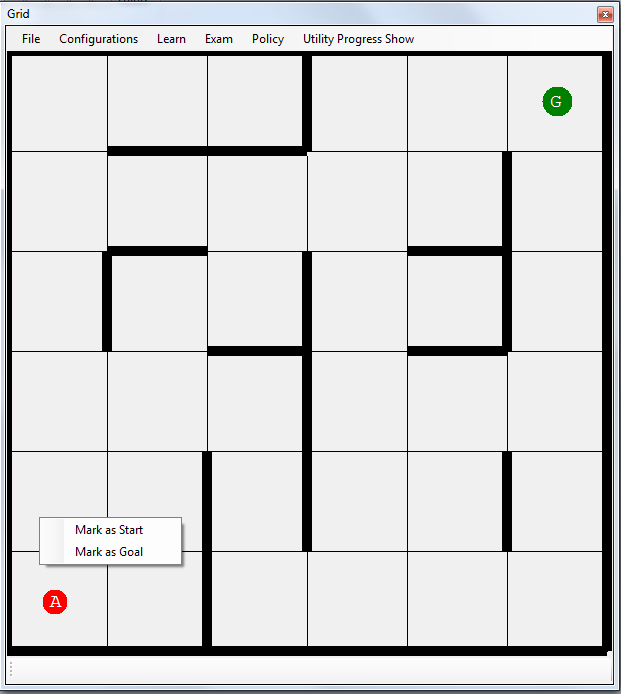
\includegraphics[width=0.5\textwidth]{init}
    \begin{center}\textarabic{
    عکس ۱: یک نمایشی از محیط برنامه که با انتخاب رو خطوط میتوان آنها را به بلوک تبدیل کرد و برعکس؛ و همچنین با راست کلیک کردن بروی خانه ها امکان انتخاب موقعیت های عامل و هدف را وجود دارد.}
    \end{center}
\end{figure}
    \subsection{\textarabic{معرفی منوهای برنامه}}
    در این قسمت به معرفی منوهای برنامه میپردازم.
        \subsubsection{File}
در منوی فایل امکان ایجاد و ذخیره کردن و بازنشانی ساختار خام محیط گذاشته شده است.
\begin{figure}[H]
    \centering
    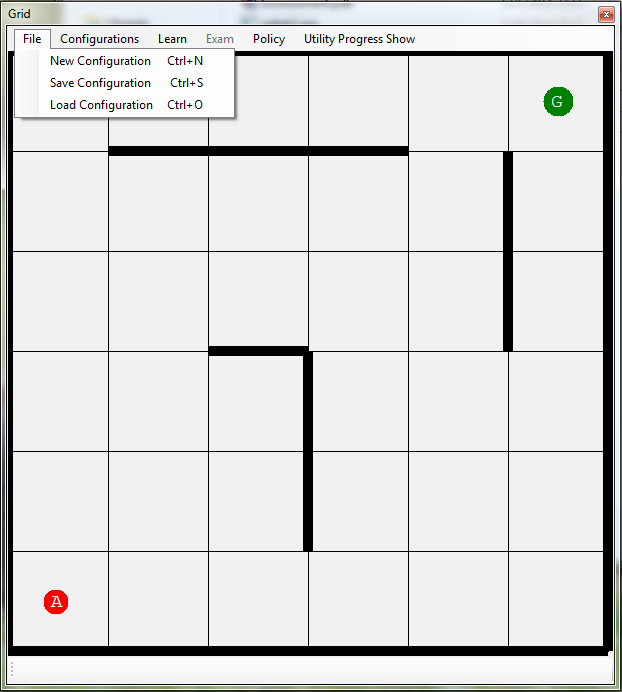
\includegraphics[width=0.5\textwidth]{file-menu}
    \begin{center}
    \textarabic{عکس ۲: منوی فایل}
    \end{center}
\end{figure}
    \subsubsection{Configurations}
    با انتخاب این منو به تنظیمات برنامه که مربوط به پارامتر های یادگیری و محیط مربوط میشود میرویم.
\begin{figure}[H]
    \centering
    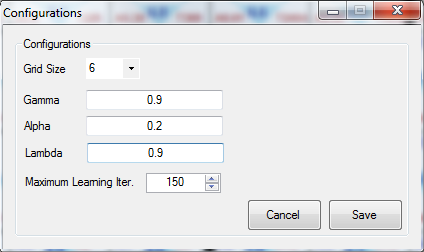
\includegraphics[width=0.5\textwidth]{conf}
    \begin{center}
    \textarabic{عکس ۳: منوی تنظیمات برنامه؛ توجه شود که اندازه شبکه همیشه مربعی در نظر گرفته شده است.}
    \end{center}
\end{figure}
    \subsubsection{Learn}
  در این منو میتوانیم یکی از ۴ الگوریتم نوشته شده را برای شبکه طراحی شده آموزش داد و نتایج بطور گرافیکی نمایش خواهند یافت که در قسمت های بعدی در مورد چگونگی تفسیر این نتایج بحث خواهد شد.
\begin{figure}[H]
    \centering
    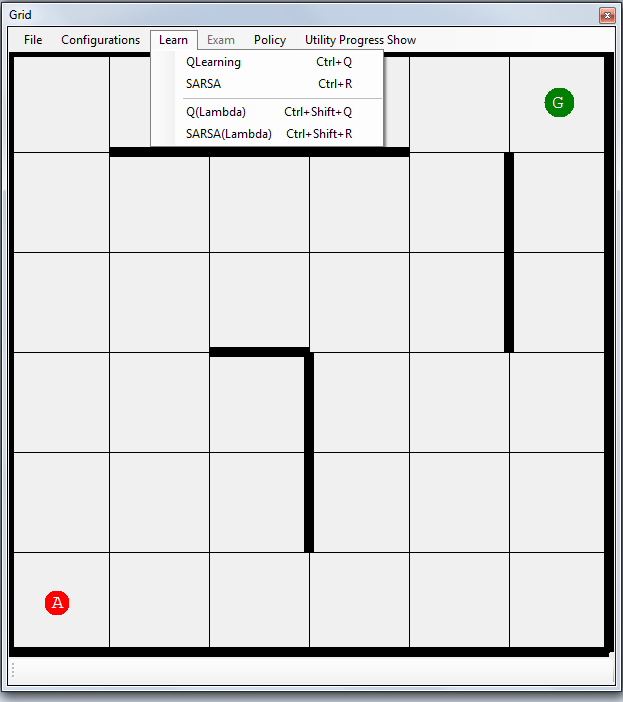
\includegraphics[width=0.5\textwidth]{learn-menu}
    \begin{center}
    \textarabic{عکس ۴: با انتخاب یکی از چهار الگوریتم؛ الگوریتم انتخاب شده شروع به یادگیری شبکه خواهد کرد.}
    \end{center}
\end{figure}
    \subsubsection{Policy}
    این منو برای ذخیره سازی و بازنشانی سیاست یادگرفته شده و سایر اطلاعاتی که پس از یادگیری شبکه بدست میاید از قبیل مقادیر سودمندی موقعیت ها و دیگر اطلاعات مرتبط مورد استفاده است که برای راحتی کار در منویی جدا قرار داده شده اند.
\begin{figure}[H]
    \centering
    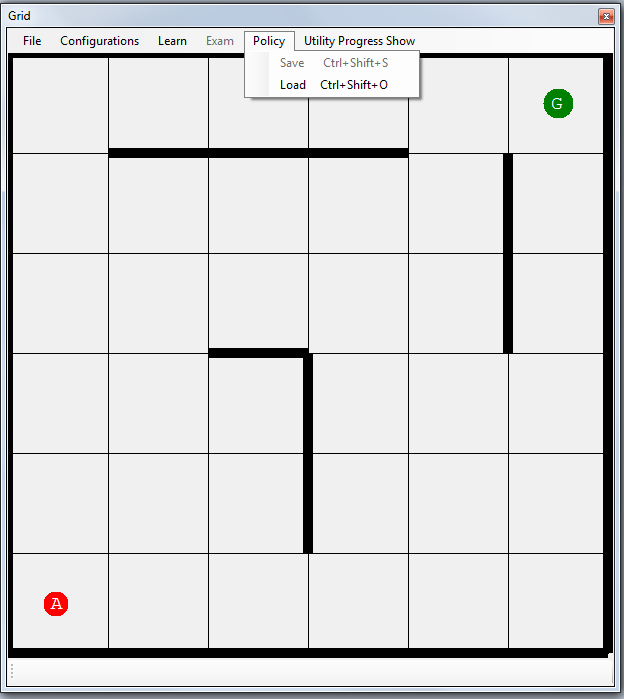
\includegraphics[width=0.5\textwidth]{policy-menu}
    \begin{center}
    \textarabic{عکس ۵: بعد از یادگیری سیاسیت و میزان سودمندی موقعیت ها میتوان آنها را ذخیره و در دفعات بعد بازنشانی کرد.}
    \end{center}
\end{figure}
    \subsubsection{Utilities Progress Show}
    برنامه در هنگام یادگیری میزان سودمندی موقعیت ها تاریخچه ای از نحوه تغییر مقادیر سودمندی تمامی موقعیت ها ذخیره میکند. که توسط این منو میتوان نحوه ی رشد یا عدم رشد سودمندی هر یک از خانه ها را به صورت جدا یا باهم(برای مقایسه) مشاهده کرد.
\begin{figure}[H]
    \centering
    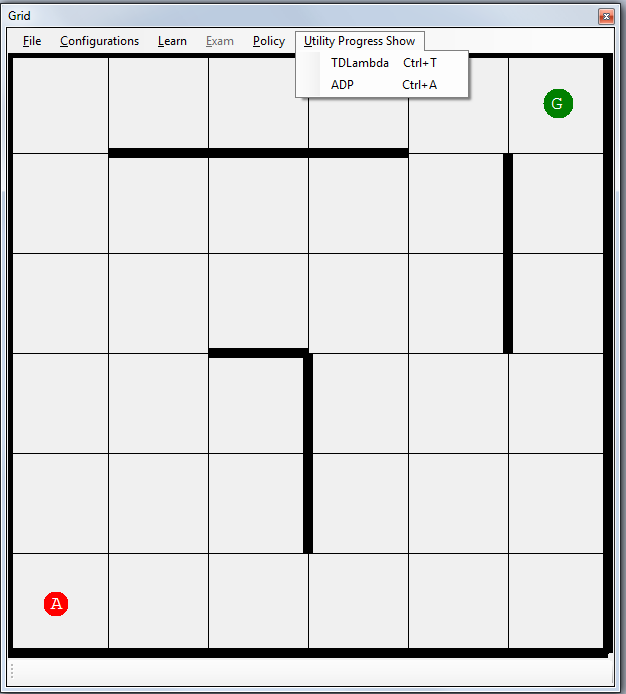
\includegraphics[width=0.5\textwidth]{util-menu}
    \begin{center}
    \textarabic{عکس ۶: با انتخاب هر یک از الگوریتم های یادگیرنده ی میزان سودمندی خانه ها میتوانیم شاهد مشاهده ی نحوه ی تغییر سودمندی موقعیت باشیم.}
    \end{center}
\end{figure}\begin{figure}[H]
    \centering
    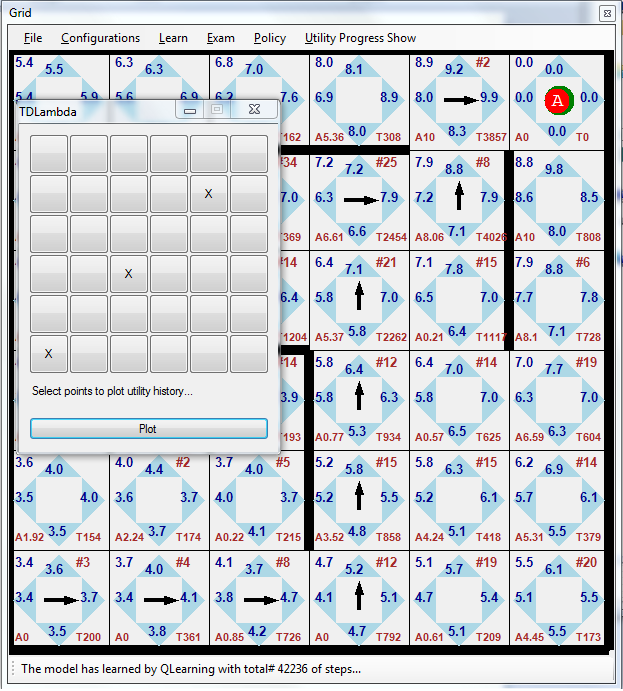
\includegraphics[width=0.5\textwidth]{util-form}
    \begin{center}
    \textarabic{عکس ۷: با انتخاب خانه های مد نظر(با هم یا به بطور تکی) می توانیم به مقایسه نحوه ی تغییر میزان سودمندی خانه ها بپردازیم.}
    \end{center}
\end{figure}
\section{\textarabic{نحوه ی نمایش داده ها}}
در نحوه ی حرکت عامل در برنامه تعریف شده است که عامل میتواند در هر موقیت تصمیم به انتخاب یکی از ۵ حرکت
\{
 شمال؛ شرق؛ جنوب؛ غرب و حفظ موقعیت
\}
نماید. که در حفظ موقعیت عامل بی حرکت می ماند.
\par
پس از یادگیری سیاست بهینه و سودمندی حالات داده های مرتبط با هر موقیت به شرح زیر در همان موقعیت نمایش داده میشوند:\\
در هر موقعیت مقدار سیاست بهینه یادگرفته شده برای چهار جهت اصلی در فلش های آبی رنگ مرتبط با همان جهت نمایش داده شده است.\\
گوشه بالایی سمت چپ هر موقعیت مقدار سیاست بهینه مربوط حرکت «حفظ موقعیت» میباشد.\\
گوشه بالایی سمت راست هر موقعیت این حقیقت را مشخص میکند که الگوریتم در آخرین مرحله یادگیری چند بار به خانه ی مورد نظر در رجوع کرده است.\\
مقدار گوشه پایینی چپ هر خانه مقدار سودمندی محاسبه شده با استفاده از برنامه نویسی پویای وفقی برای آن موقیعت را نمایش میدهد و متعاقبا گوشه پایینی راست هر خانه مقدار سومندی آن خانه که توسط روش
\textenglish{$TD(\lambda)$}
حساب شده است را نمایش میدهد.
\footnote{\textarabic{توجه شود که در برنامه نویسی این برنامه مبدا مختصات موقعیت های شبکه را گوشه بالایی سمت چپ در نظر گرفته شده است ولی با توجه به متن تمرین داده شده میتوان این را نتیجه گرفت که مبدا مختصات گوشه پایینی سمت چپ است؛ بنابراین ایندکس های خانه های چاپ شده با توجه یه مبدا مختصات برنامه یعنی گوشه بالایی سمت چپ در نظر گرفته شده است.}}



\section{\textarabic{اجرای برنامه}}
شبکه درخواست شده در متن تکلیف توسط ۴ الگوریتم معرفی شده در مقدمه این متن مورد یادگیری قرار گرفته است. که شرح نتایج آنها به صورت زیر است.

\subsection{$Q(s, a)$}

\end{Arabic}
\begin{figure}[H]
    \centering
    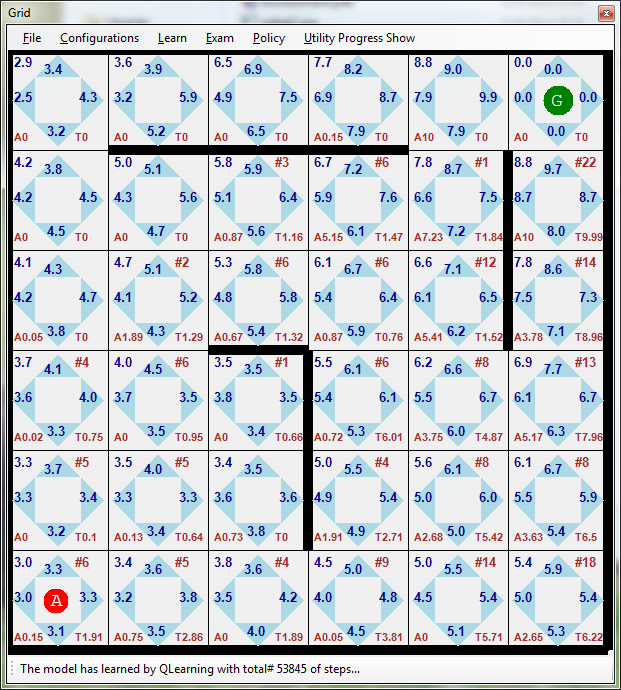
\includegraphics[width=0.5\textwidth]{q}
    \begin{center}
    \textarabic{عکس ۸: سیاست و میزان سودمندی های یادگرفته شده توسط الگوریتم $Q(s, a)$ }
    \end{center}
\end{figure}
\newpage
\begin{figure}[h]
        \centering
        \begin{subfigure}[b]{0.5\textwidth}
            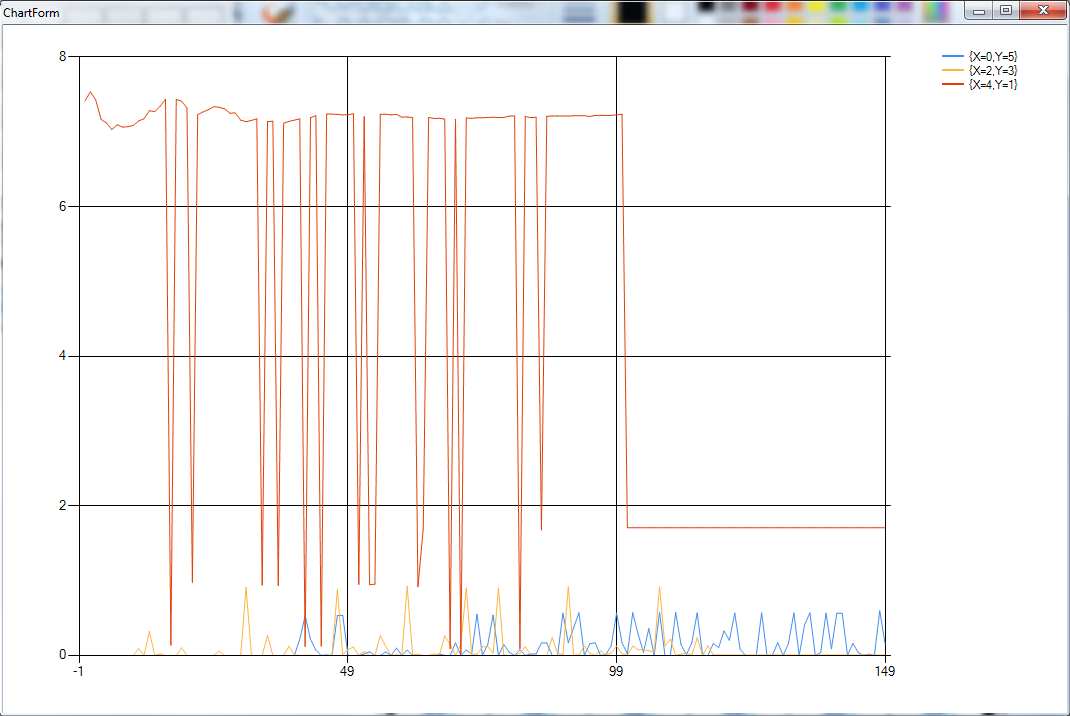
\includegraphics[width=\textwidth]{q-adp}
            \begin{center}
                \textarabic{ب: روند تغییر مقاریر سودمندی یادگرفته شده توسط روش $ADP$ }
            \end{center}
        \end{subfigure}%
        ~ %add desired spacing between images, e. g. ~, \quad, \qquad, \hfill etc.
          %(or a blank line to force the subfigure onto a new line)
        \begin{subfigure}[b]{0.5\textwidth}
           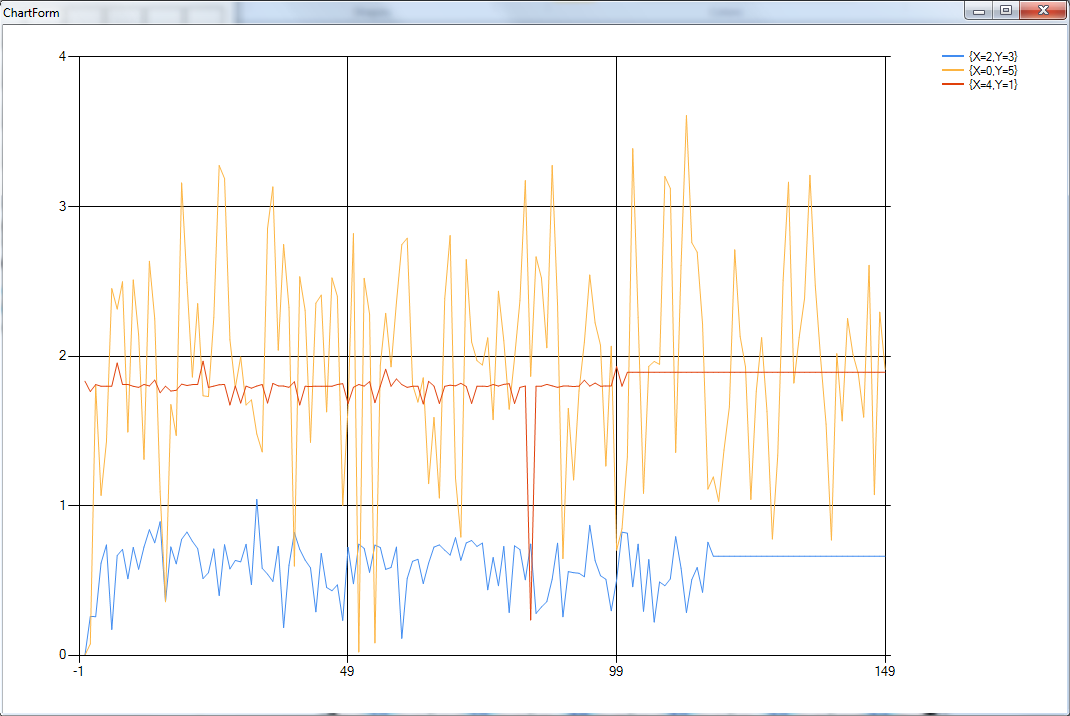
\includegraphics[width=\textwidth]{q-td}
            \begin{center}
                \textarabic{الف: روند تغییر مقادیر سودمندی یادگرفته شده توسط روش $TD(\lambda)$ }
            \end{center}
        \end{subfigure}
    \begin{center}
    \textarabic{عکس ۹: روند تغییر مقدریر سودمندی یادگرفته شده توسط روش های
     $TD(\lambda)$ و $ADP$
      برای خانه های 
     $(1, 1)$, $(3,3)$ 
     و
      $(5, 5)$
     }
    \end{center}
\end{figure}

\begin{figure}[H]
    \centering
    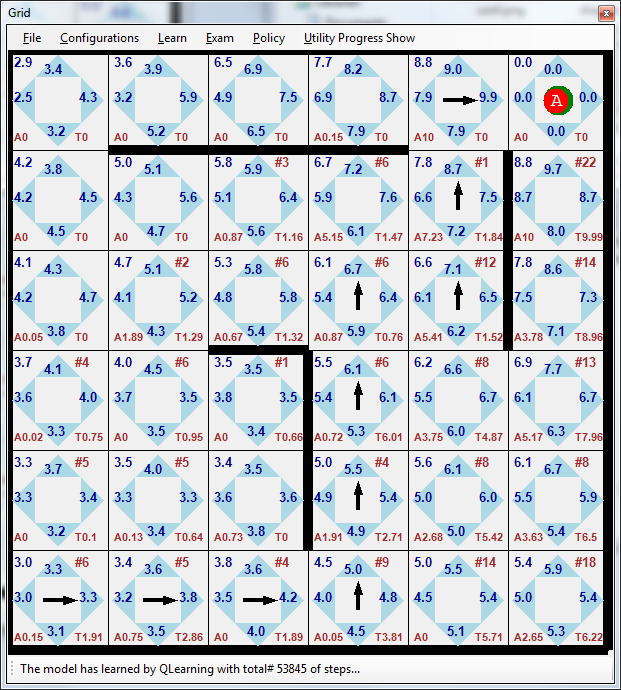
\includegraphics[width=0.5\textwidth]{q-exec}
    \begin{center}
    \textarabic{عکس ۱۰: مسیر طی شده توسط عامل با توجه به سیاست یادگرفته شده توسط الگوریتم $Q(s, a)$ }
    \end{center}
\end{figure}

\subsection{$SARSA(s, a)$}

\begin{figure}[H]
    \centering
    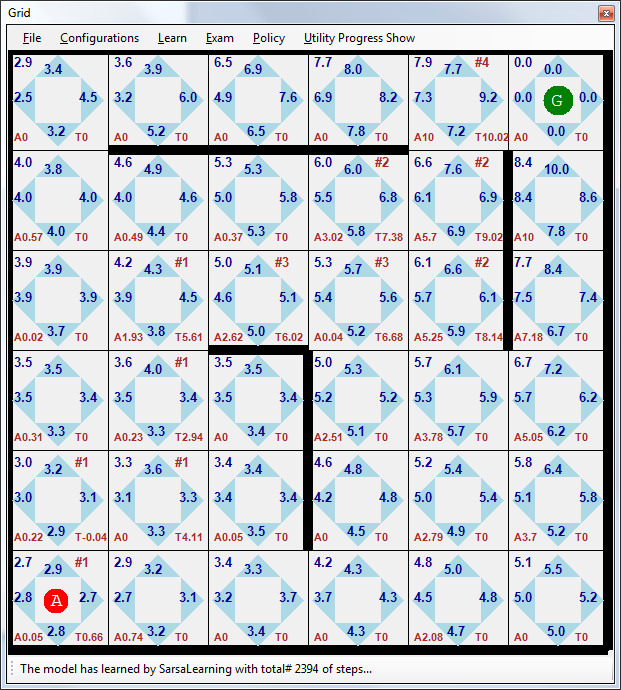
\includegraphics[width=0.5\textwidth]{r}
    \begin{center}
    \textarabic{عکس ۱۱: سیاست و میزان سودمندی های یادگرفته شده توسط الگوریتم $SARSA(s, a)$ }
    \end{center}
\end{figure}
\begin{figure}[h]
        \centering
        \begin{subfigure}[b]{0.5\textwidth}
            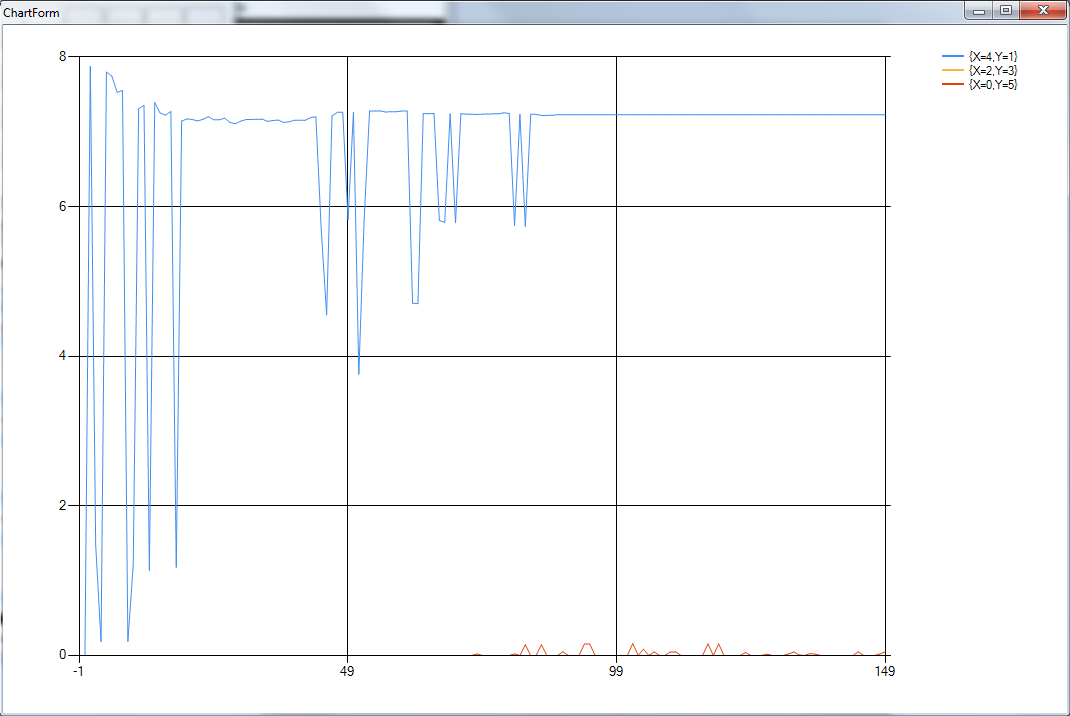
\includegraphics[width=\textwidth]{r-adp}
            \begin{center}
                \textarabic{ب: روند تغییر مقاریر سودمندی یادگرفته شده توسط روش $ADP$ }
            \end{center}
        \end{subfigure}%
        ~ %add desired spacing between images, e. g. ~, \quad, \qquad, \hfill etc.
          %(or a blank line to force the subfigure onto a new line)
        \begin{subfigure}[b]{0.5\textwidth}
           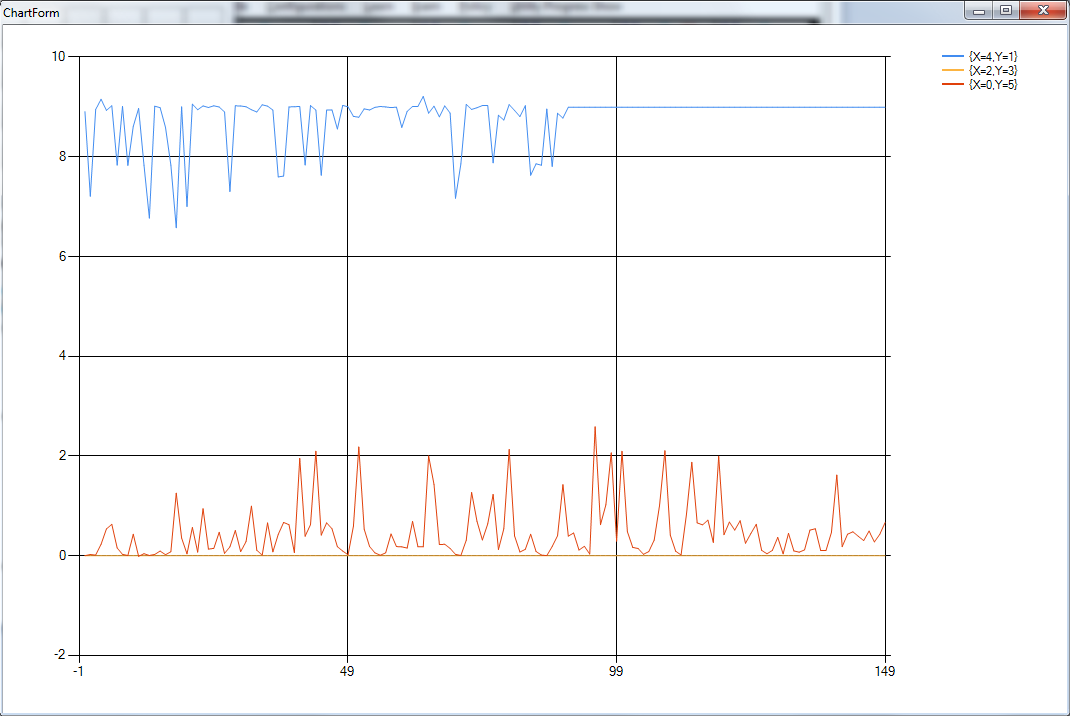
\includegraphics[width=\textwidth]{r-td}
            \begin{center}
                \textarabic{الف: روند تغییر مقادیر سودمندی یادگرفته شده توسط روش $TD(\lambda)$ }
            \end{center}
        \end{subfigure}
    \begin{center}
    \textarabic{عکس ۱۲: روند تغییر مقدریر سودمندی یادگرفته شده توسط روش های
     $TD(\lambda)$ و $ADP$
      برای خانه های 
          $(1, 1)$, $(3,3)$ 
     و
      $(5, 5)$
     }
    \end{center}
\end{figure}

\begin{figure}[H]
    \centering
    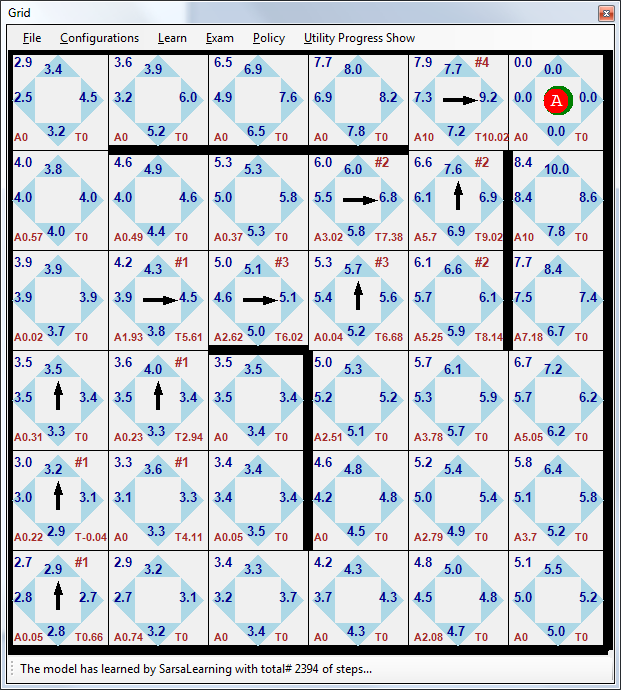
\includegraphics[width=0.5\textwidth]{r-exec}
    \begin{center}
    \textarabic{عکس ۱۳: مسیر طی شده توسط عامل با توجه به سیاست یادگرفته شده توسط الگوریتم $SARSA(s, a)$ }
    \end{center}
\end{figure}


\subsection{$Q(\lambda)$}

\begin{figure}[H]
    \centering
    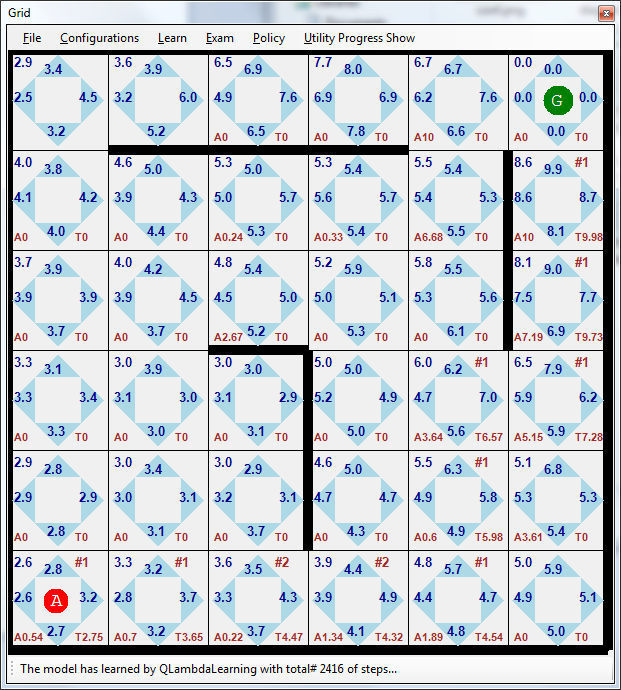
\includegraphics[width=0.5\textwidth]{qlambda}
    \begin{center}
    \textarabic{عکس ۱۴: سیاست و میزان سودمندی های یادگرفته شده توسط الگوریتم $Q(\lambda)$ }
    \end{center}
\end{figure}
\begin{figure}[h]
        \centering
        \begin{subfigure}[b]{0.5\textwidth}
            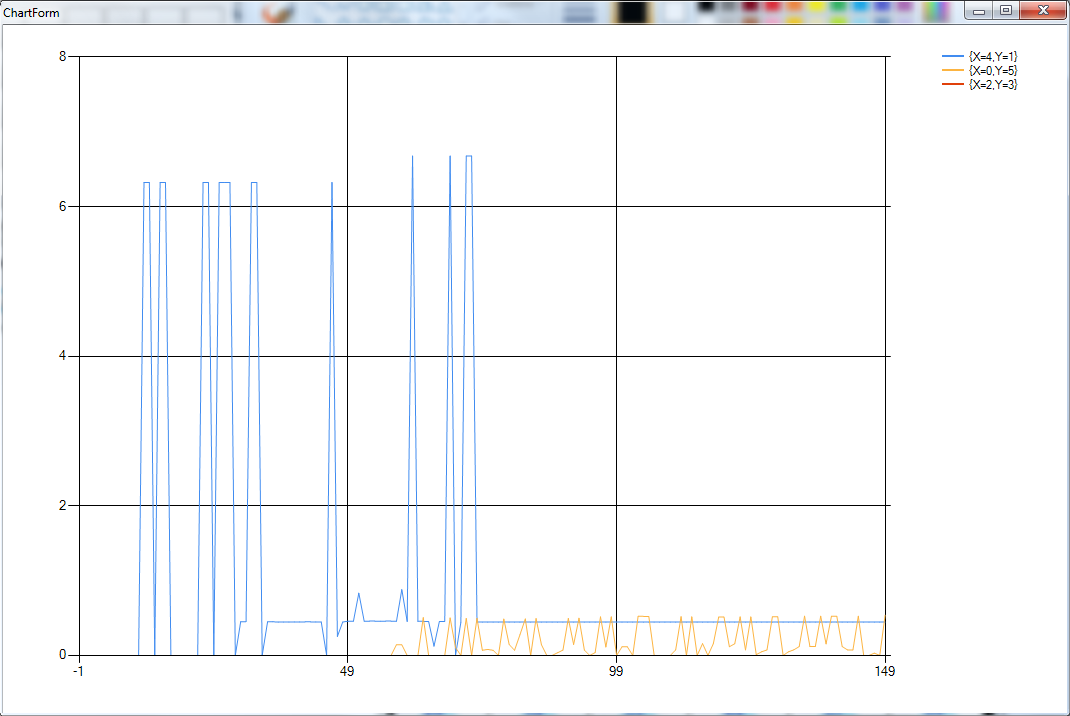
\includegraphics[width=\textwidth]{qlambda-adp}
            \begin{center}
                \textarabic{ب: روند تغییر مقاریر سودمندی یادگرفته شده توسط روش $ADP$ }
            \end{center}
        \end{subfigure}%
        ~ %add desired spacing between images, e. g. ~, \quad, \qquad, \hfill etc.
          %(or a blank line to force the subfigure onto a new line)
        \begin{subfigure}[b]{0.5\textwidth}
           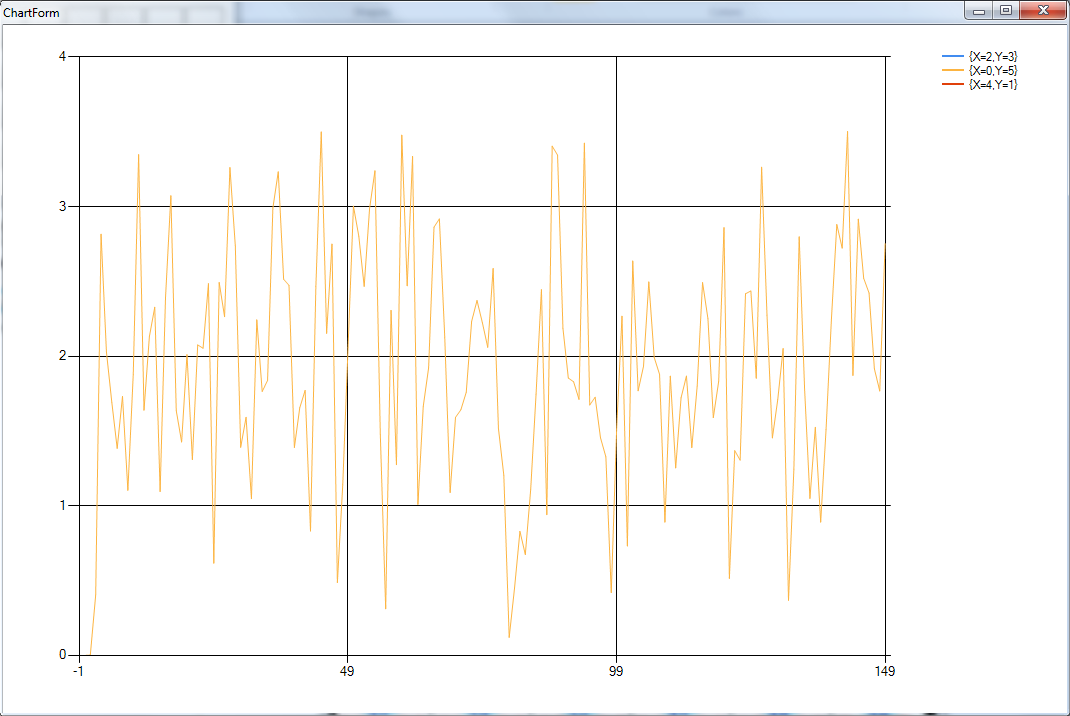
\includegraphics[width=\textwidth]{qlambda-td}
            \begin{center}
                \textarabic{الف: روند تغییر مقادیر سودمندی یادگرفته شده توسط روش $TD(\lambda)$ }
            \end{center}
        \end{subfigure}
    \begin{center}
    \textarabic{عکس ۱۵: روند تغییر مقدریر سودمندی یادگرفته شده توسط روش های
     $TD(\lambda)$ و $ADP$
      برای خانه های 
      $(1, 1)$, $(3,3)$ 
     و
      $(5, 5)$     }
    \end{center}
\end{figure}

\begin{figure}[H]
    \centering
    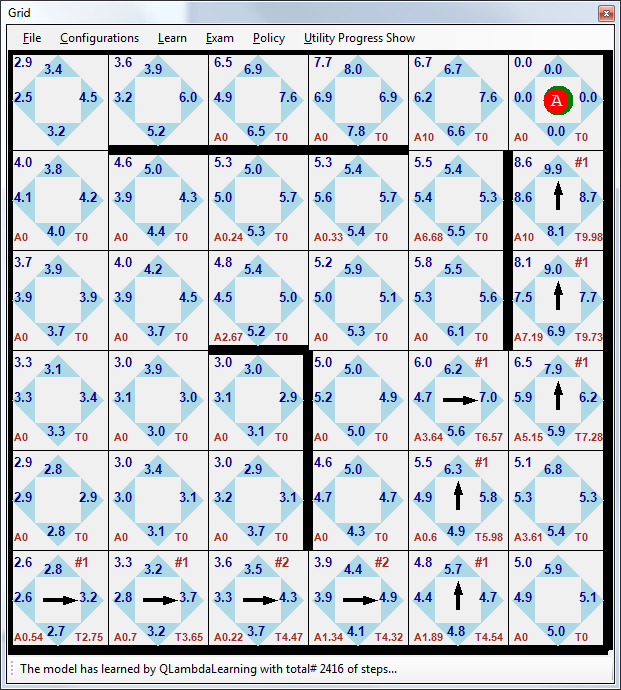
\includegraphics[width=0.5\textwidth]{qlambda-exec}
    \begin{center}
    \textarabic{عکس ۱۶: مسیر طی شده توسط عامل با توجه به سیاست یادگرفته شده توسط الگوریتم $Q(\lambda)$ }
    \end{center}
\end{figure}
\subsection{$SARSA(\lambda)$}

\begin{figure}[H]
    \centering
    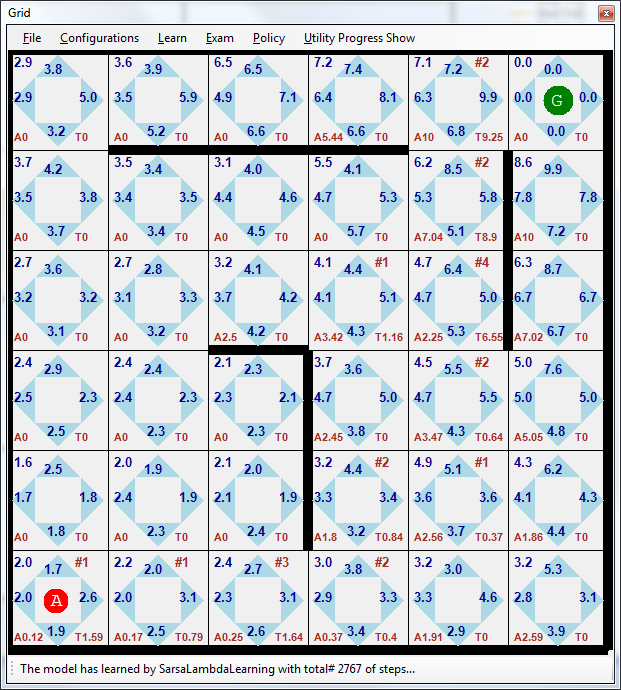
\includegraphics[width=0.5\textwidth]{rlambda}
    \begin{center}
    \textarabic{عکس ۱۷: سیاست و میزان سودمندی های یادگرفته شده توسط الگوریتم $SARSA(\lambda)$ }
    \end{center}
\end{figure}
\begin{figure}[h]
        \centering
        \begin{subfigure}[b]{0.5\textwidth}
            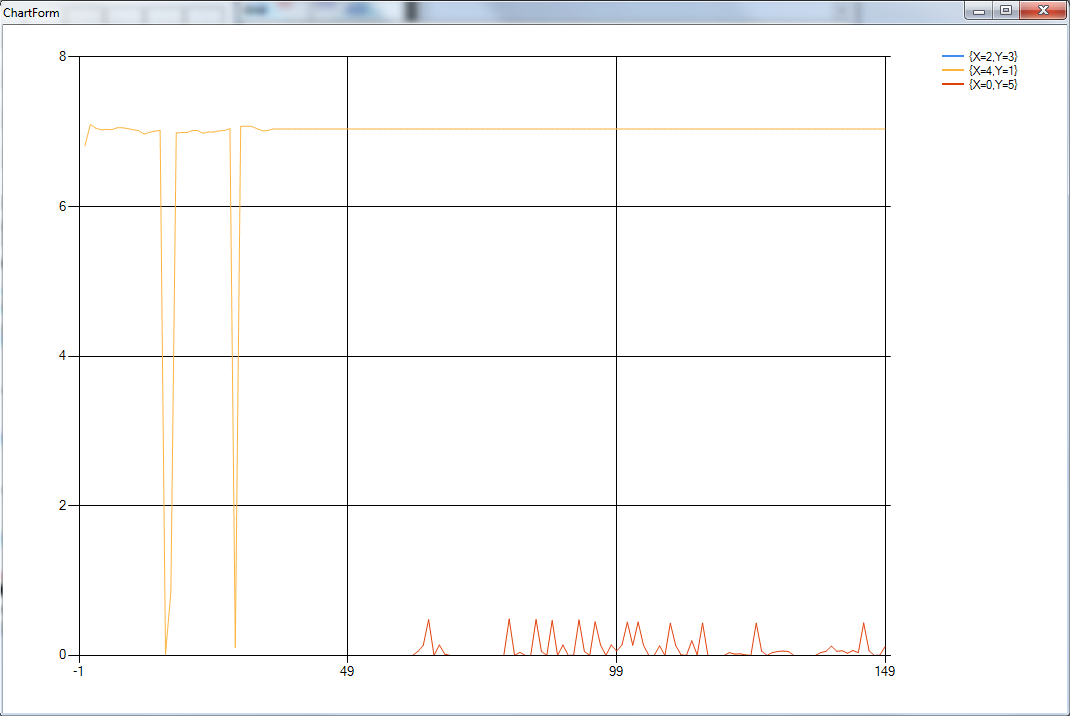
\includegraphics[width=\textwidth]{rlambda-adp}
            \begin{center}
                \textarabic{ب: روند تغییر مقاریر سودمندی یادگرفته شده توسط روش $ADP$ }
            \end{center}
        \end{subfigure}%
        ~ %add desired spacing between images, e. g. ~, \quad, \qquad, \hfill etc.
          %(or a blank line to force the subfigure onto a new line)
        \begin{subfigure}[b]{0.5\textwidth}
           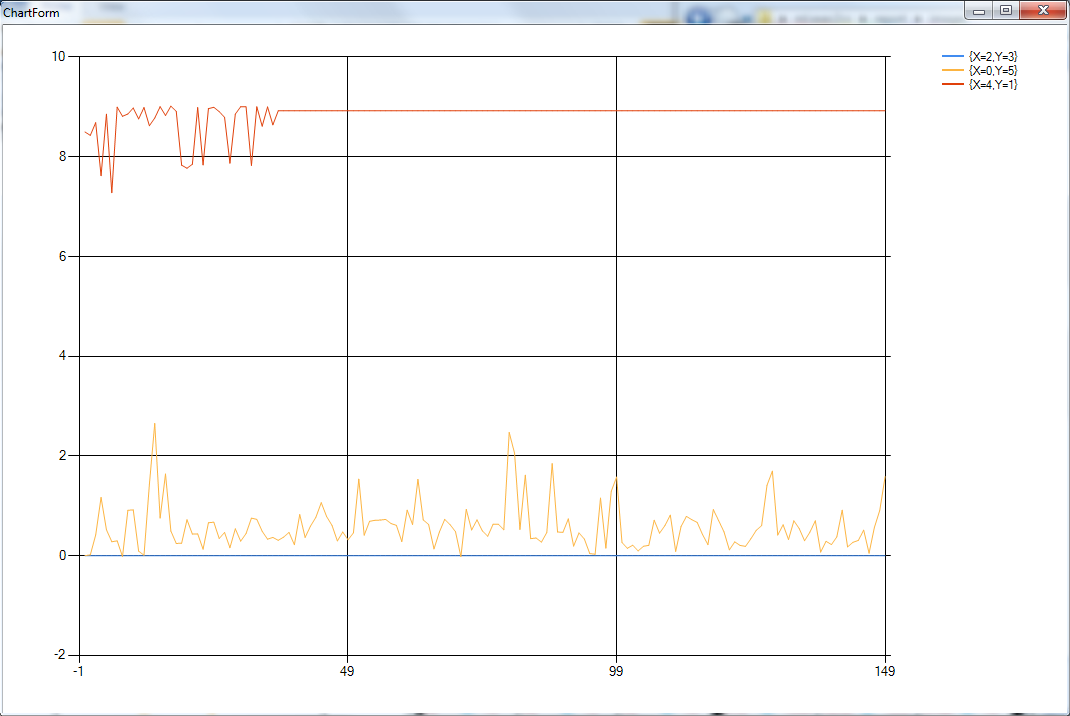
\includegraphics[width=\textwidth]{rlambda-td}
            \begin{center}
                \textarabic{الف: روند تغییر مقادیر سودمندی یادگرفته شده توسط روش $TD(\lambda)$ }
            \end{center}
        \end{subfigure}
    \begin{center}
    \textarabic{عکس ۱۸: روند تغییر مقدریر سودمندی یادگرفته شده توسط روش های
     $TD(\lambda)$ و $ADP$
      برای خانه های 
      $(1, 1)$, $(3,3)$ 
     و
      $(5, 5)$
     }
    \end{center}
\end{figure}

\begin{figure}[H]
    \centering
    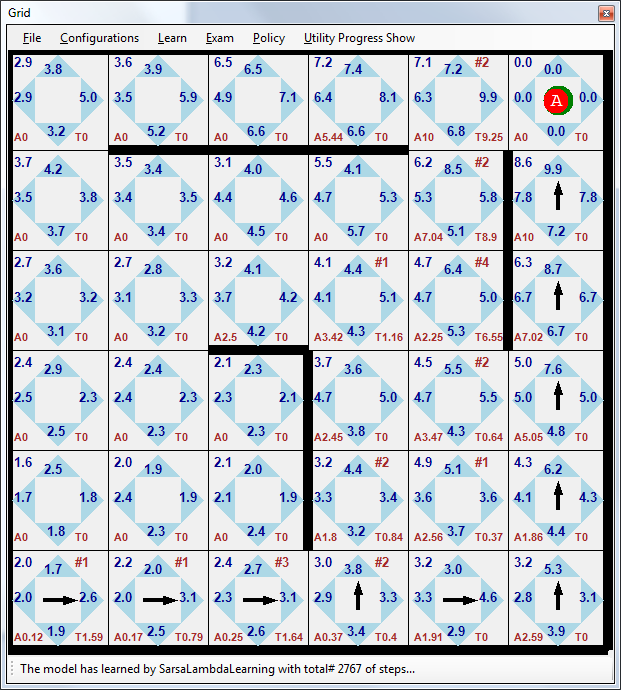
\includegraphics[width=0.5\textwidth]{rlambda-exec}
    \begin{center}
    \textarabic{عکس ۱۹: مسیر طی شده توسط عامل با توجه به سیاست یادگرفته شده توسط الگوریتم $SARSA(\lambda)$ }
    \end{center}
\end{figure}

\begin{Arabic}
\section{\textarabic{توضیحاتی در مورد برنامه نویسی شی گرا و اشیا برنامه}}
همان طور که میدانیم
\textenglish{C\#}
یک زبان مبتنی بر برنامه نویسی شی گرا میباشد. بنده برای پیاده سازی این برنامه در ابتدا به نوشتن ۲ عدد کتابخانه اقدام کردم یکی برای مدل کردن محیط و اعملیات های مرتبط با محیط و دیگری برای الگوریتم های یادگیری محیط میباشد. برنامه اصلی(اجرایی) از هر دوی این کتابخانه ها استفاده میکند و مدل انتزاعی محیط را به محیط گرافیکی تبدیل میکند. و با تحویل محیط انتزاعی به الگوریتم های یادگیری تقویتی نوشته شده در دیگر کتابخانه یک هماهنگی و ارتباط بین این دو ایجاد میکند.

\subsection{\textarabic{کتابخانه محیط}}
این کتابخانه امکانات کافی برای انتزاع محیط واقعی را در اختیارمان میگذارد. و همچنین قابلیت تبدیل مدل گرافیکی به مدل انتزاع وبرعکس را دارد. که در هنگام ذخیره و بازنشانی شبکه کاربرد دارد. نمودار کلاس های مرتبط با این کتابخانه در شکل شماره ۲۰ آمده است.

\begin{figure}[H]
    \centering
    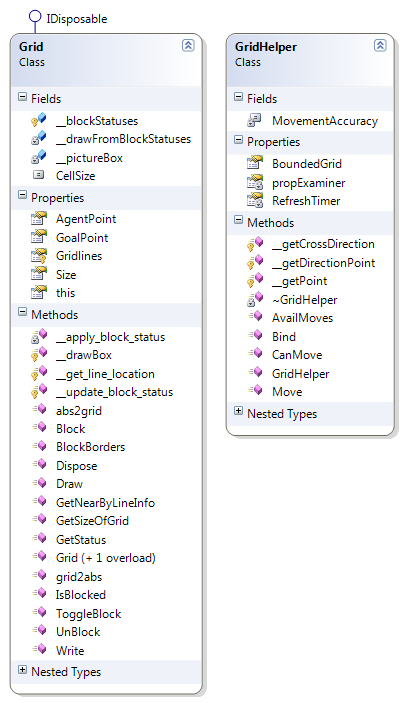
\includegraphics[width=0.5\textwidth]{diag-env}
    \begin{center}
    \textarabic{عکس ۲۰: نمودار کلاسی کتابخانه ی محیط}
    \end{center}
\end{figure}

\subsection{\textarabic{کتابخانه یادگیری تقویتی}}
در این کتابخانه صرفا پیاده سازی الگوریتم های یادگیری تقویتی که در بخش مقدمه معرفی شده اند آمده اند. این کتابخانه از کتابخانه محیط برای اعمال امور مربوط به محیط از قبل شبیه سازی کردن جابجایی انتزاعی عامل در طی روند یادگیری و ... استفاده میکند. به علت در نظر گرفتن طراحی صحیح از نحوه ی اشتقاق کلاس های این کتابخانه؛ در پیاده سازی هر یک از الگوریتم ها فقط کافی است که متد های 
\textenglish{Learn()}
و
\textenglish{\char`_\char`_update\char`_q\char`_value()}
مربوط به آن الگوریتم ها را پیاده سازی کنیم. مابقی مسايل بطور خودکار انجام خواهند شد. نمودار کلاسی کتابخانه ی یادگیری تقویتی در شکل شماره ۲۱ آمده است.(به نحوه ی اشتقاق گیری و توابع کلاس های پدر توجه شود.)
\newpage
\begin{sidewaysfigure}
\begin{figure}[H]
    \centering
    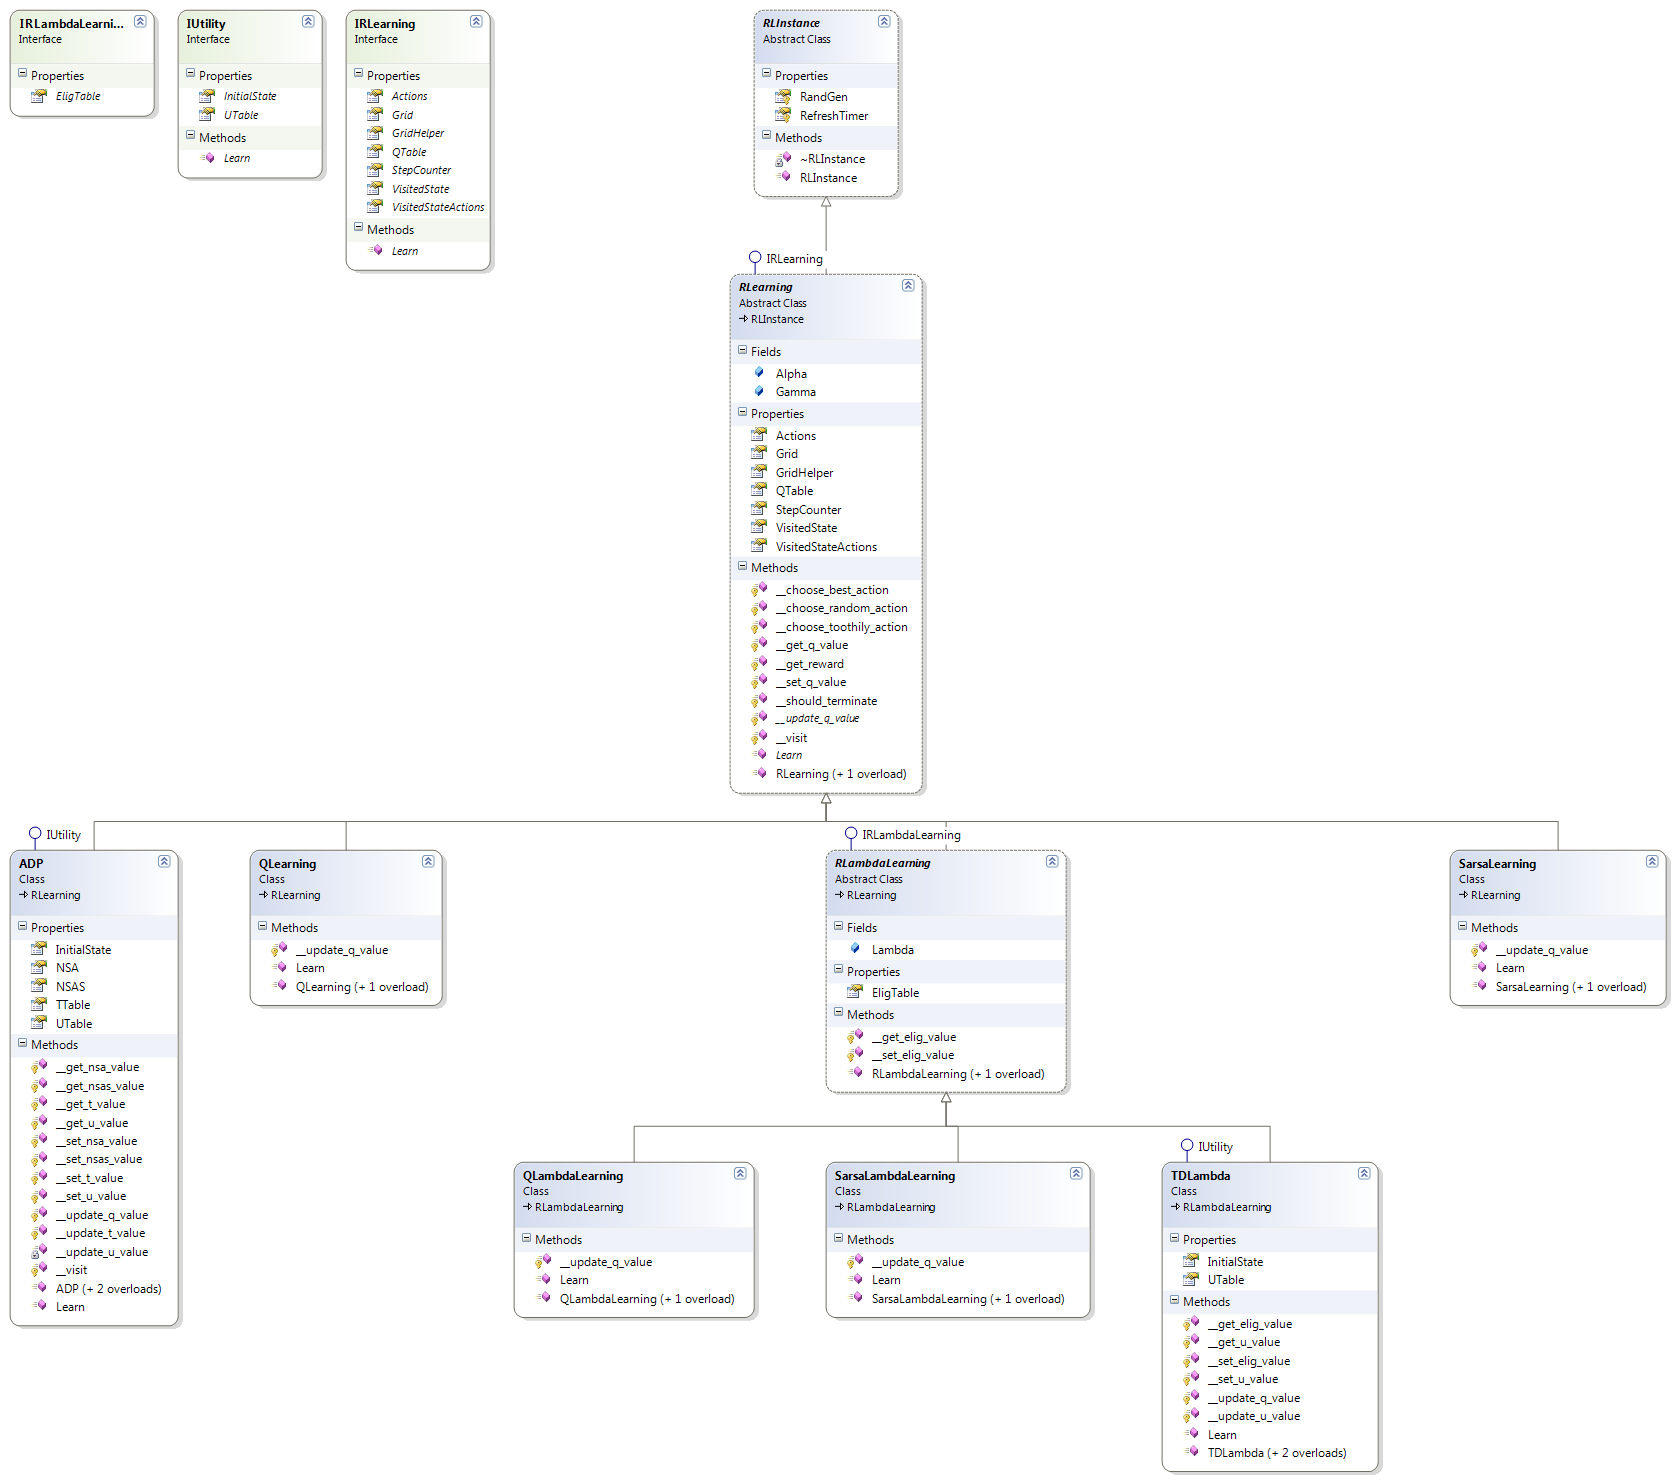
\includegraphics[width=\textwidth]{diag-rl}
    \begin{center}
    \textarabic{عکس ۲۱: نمودار کلاسی کتابخانه ی یادگیری تقویتی}
    \end{center}
\end{figure}
\end{sidewaysfigure}
\clearpage

\subsection{\textarabic{برنامه ی اجرایی}}
برنامه اجرایی در واقع پل رابطی بین دو کتابخانه محیط و یادگیری تقویتی میباشد. و همچنین برنامه ی اجرایی است که بستر مناسب برای ظاهری گرافیکی برنامه را فراهم میکند.
\begin{figure}[H]
    \centering
    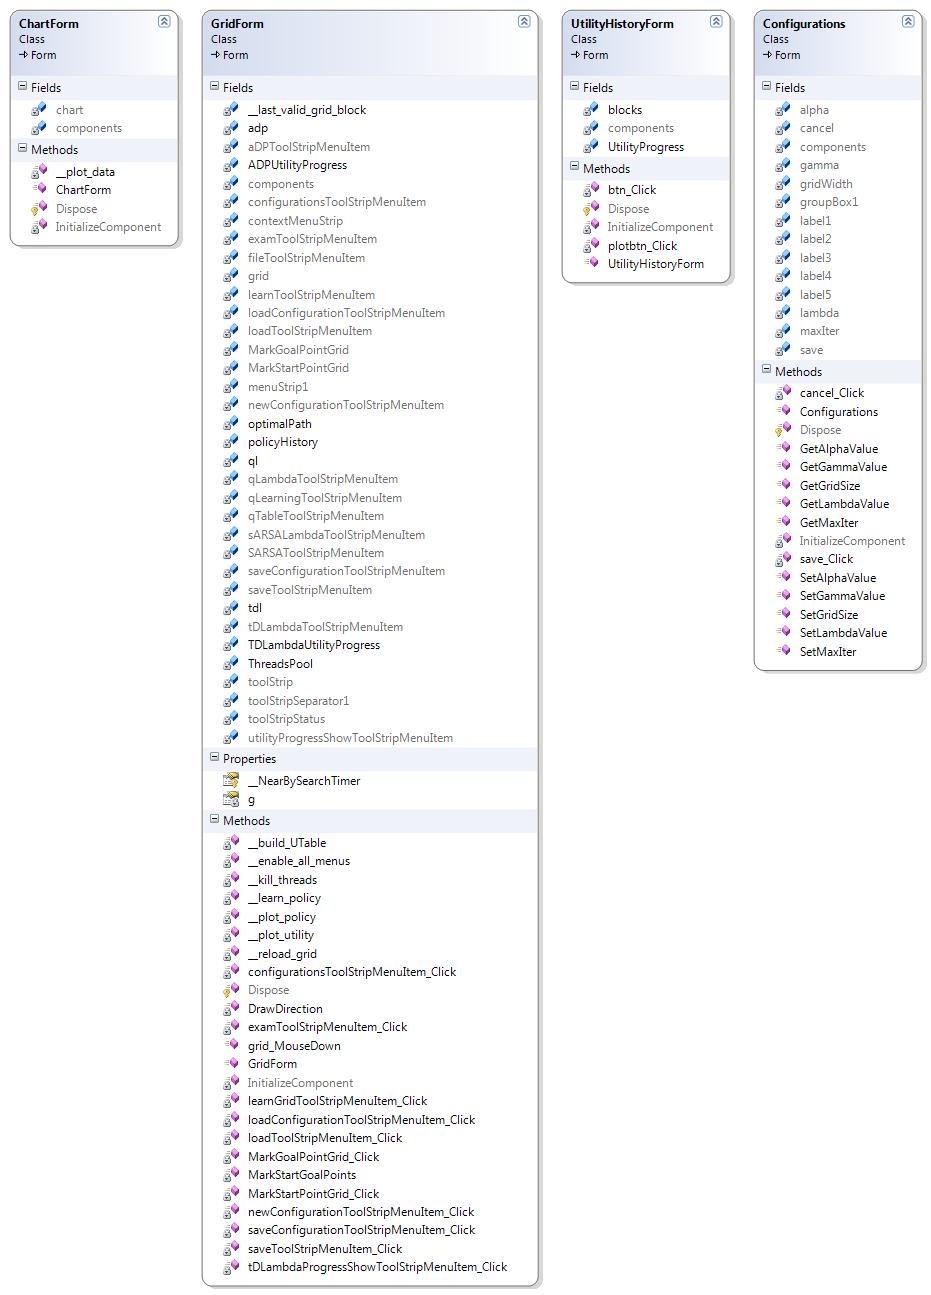
\includegraphics[width=.75\textwidth]{diag-form}
    \begin{center}
    \textarabic{عکس ۲۲: نمودار کلاسی برنامه اجرایی}
    \end{center}
\end{figure}
\end{Arabic}
\end{document}
